\documentclass[xcolor=x11names, compress]{beamer}

%% General document %%%%%%%%%%%%%%%%%%%%%%%%%%%%%%%%%%
\usepackage{graphicx}
\graphicspath{{graphics/}}

\usepackage{tikz}
\usepackage{color}
\input{rgb}

\definecolor{capri}{rgb}{0,.75,1}
\definecolor{coral}{rgb}{1,.2,.2}

\newcommand{\hltyellow}[1]{\colorbox{yellow}{$\displaystyle #1$}}
\newcommand{\hltblue}[1]{\colorbox{capri}{$\displaystyle #1$}}
\newcommand{\hltred}[1]{\colorbox{coral}{$\displaystyle #1$}}
\newcommand{\hltgreen}[1]{\colorbox{green}{$\displaystyle #1$}}

\usepackage{hyperref}

\usepackage{ulem}
\renewcommand<>{\sout}[1]{
  \only#2{\beameroriginal{\sout}{#1}}
  \invisible#2{#1}
}

%%%%%%%%%%%%%%%%%%%%%%%%%%%%%%%%%%%%%%%%%%%%%%%%%%%%%%

%% Beamer Layout %%%%%%%%%%%%%%%%%%%%%%%%%%%%%%%%%%
% \usetheme{Madrid}

\useoutertheme[subsection=false,shadow]{miniframes}
\useinnertheme{default}
\usefonttheme{serif}
\usepackage{palatino}

\setbeamerfont{title like}{shape=\scshape}
\setbeamerfont{frametitle}{shape=\scshape, series = \bfseries}
\setbeamertemplate{frametitle}[default][center]
\setbeamerfont{footnote}{size=\tiny}
\addtobeamertemplate{footnote}{}{\vspace{1ex}} %so that the footnotes do not overlap with navigation symbols at bottom

\setbeamercolor*{lower separation line head}{bg=DeepSkyBlue4} 
\setbeamercolor*{normal text}{fg=black,bg=white} 
\setbeamercolor*{alerted text}{fg=red} 
\setbeamercolor*{example text}{fg=black} 
\setbeamercolor*{structure}{fg=black}
 
\setbeamercolor*{palette tertiary}{fg=black,bg=black!10} 
\setbeamercolor*{palette quaternary}{fg=black,bg=black!10} 

\renewcommand{\(}{\begin{columns}}
\renewcommand{\)}{\end{columns}}
\newcommand{\<}[1]{\begin{column}{#1}}
\renewcommand{\>}{\end{column}}

\def\signed #1{{\leavevmode\unskip\nobreak\hfil\penalty50\hskip2em
  \hbox{}\nobreak\hfil(#1)%
  \parfillskip=0pt \finalhyphendemerits=0 \endgraf}}

\newsavebox\mybox
\newenvironment{aquote}[1]
  {\savebox\mybox{#1}\begin{quote}}
  {\signed{\usebox\mybox}\end{quote}}

%%%%%%%%%%%%%%%%%%%%%%%%%%%%%%%%%%%%%%%%%%%%%%%%%%%%

\begin{document}

%%%%%%%%%%%%%%%%%%%%%%%%%%%%%%%%%%%%%%%%%%%%%%%%%%%%%%
{
  \usebackgroundtemplate{\includegraphics[width=\paperwidth]{back.jpg}}
\begin{frame}[plain]

  \vspace{100pt}
  \title{\bf The Metabolic basis of Ecological and Evolutionary Dynamics}
  \subtitle{A MulaQuaBio Lecture}
 
\titlepage
\date{}

\end{frame}
}
%%%%%%%%%%%%%%%%%%%%%%%%%%%%%%%%%%%%%%%%%%%%%%%%%%%%%%
\section{\scshape Introduction}
% \subsection{}
%%%%%%%%%%%%%%%%%%%%%%%%%%%%%%%%%%%%%%%%%%%%%%%%%%%%%%

\begin{frame}{Outline}
  \begin{itemize}\setlength{\itemindent}{0em}\itemsep12pt

    \item Introduction

    \item Energy and Metabolic rate

		\item Importance of Body Size
		
		\item Importance of Temperature

    \item Summary, Questions, and Readings

  \end{itemize}  

\end{frame}
% %%%%%%%%%%%%%%%%%%%%%%%%%%%%%%%%%%%%%%%%%%%%%%%%%%%%%%

\begin{frame}{The importance of metabolism in Ecology}

\begin{columns}[c]
  \column{0.3\textwidth}\centering
    \vspace*{\fill} \includegraphics[width=\textwidth]{Boltz.jpg} 
    {\tiny By Unknown author - Universit\"{a}t Wien, Public Domain, \url{https://commons.wikimedia.org/w/index.php?curid=867246}\par}\vspace*{\fill}  
  \column{0.7\textwidth}\centering
  \vspace*{\fill} 
  \begin{quote} 
  The 'struggle for existence' of living beings is not for the fundamental constituents of food ... but for the possession of the free energy obtained, chiefly by means of the green plant, from the transfer of radiant energy from the hot sun to the cold earth. \\
  \centering
    \hfill -- {\small Ludwig Boltzmann 1886, ``The Second Law of Thermodynamics''}
\end{quote}
\vspace*{\fill}
\end{columns}

\pause

\vspace*{\fill}
\centering {\it Read Brown et al (2004), ``Toward a metabolic theory of ecology''}
\vspace*{\fill}

\end{frame}

%%%%%%%%%%%%%%%%%%%%%%%%%%%%%%%%%%%%%%%%%%%%%%%%%%%%%%

\begin{frame}{The importance of metabolism in ecology}

\begin{itemize}[<+->]\setlength{\itemindent}{0em} \itemsep20pt
  \item Ecosystems are complex
	\vspace{5pt}
	\begin{columns}[c]
	  \column{0.5\textwidth}
	    \includegraphics[width=\linewidth]{graphics/Reef.jpg}
	  \column{0.5\textwidth}
	    \includegraphics[width=0.94\linewidth]{graphics/Rainforest.jpg}
	\end{columns}

	\item \textit{A {\bf metabolic} (AKA ``bottom-up'' or ''mechanistic'')  
	understanding of these complex ecosystems is necessary}
\end{itemize}
    
\end{frame}

%%%%%%%%%%%%%%%%%%%%%%%%%%%%%%%%%%%%%%%%%%%%%%%%%%%%%%
\begin{frame}{A metabolic ecology roadmap}

\begin{tikzpicture}
  \node (img1) {\includegraphics[width=4.2in]{Roadmap1.png}};
  \pause
  \node (img2) at (img1) {\includegraphics[width=4.2in]{Roadmap2.png}};
  \pause
  \node (img3) at (img1) {\includegraphics[width=4.2in]{Roadmap9.png}};
  \pause
  \node (img4) at (img1) {\includegraphics[width=4.2in]{Roadmap3.png}};
  \pause
  \node (img5) at (img1) {\includegraphics[width=4.2in]{Roadmap4.png}};
  \pause
  \node (img6) at (img1) {\includegraphics[width=4.2in]{Roadmap5.png}};
  \pause
  \node (img7) at (img1) {\includegraphics[width=4.2in]{Roadmap6.png}};
  \pause
  \node (img8) at (img1) {\includegraphics[width=4.2in]{Roadmap7.png}};
  \pause
  \node (img9) at (img1) {\includegraphics[width=4.2in]{Roadmap8.png}};
  \pause
  \node (img10) at (img1) {\includegraphics[width=4.2in]{Roadmap10.png}};
  \pause
  \node (img11) at (img1) {\includegraphics[width=4.2in]{Roadmap11.png}};
  \pause
  \node (img12) at (img1) {\includegraphics[width=4.2in]{Roadmap12.png}};

\end{tikzpicture}

\begin{itemize}[<+->]\setlength{\itemindent}{0em} \itemsep10pt
  \item Individual-level {\it energy use and metabolic rate} determines:
		\begin{itemize}\setlength{\itemindent}{0em} \itemsep6pt
			\item Population growth rate (a measure of the population's fitness)
			\item Interaction rates with other individuals (including consumption
			rates - another lecture)
		\end{itemize}
\end{itemize}

\end{frame}

%%%%%%%%%%%%%%%%%%%%%%%%%%%%%%%%%%%%%%%%%%%%%%%%%%%%%%
\section{\scshape Energy and metabolic rate}
% \subsection{}

%%%%%%%%%%%%%%%%%%%%%%%%%%%%%%%%%%%%%%%%%%%%%%%%%%%%%%
\begin{frame}{Energy and Metabolic rate}
\begin{center}
  \begin{tikzpicture}
    \node (img1) {\includegraphics[width=4.2in]{Roadmap1.png}};
  \end{tikzpicture}
\end{center}
\begin{itemize}[<+->]\setlength{\itemindent}{0em}
  \item We will focus on the first ``stop'' on this roadmap in this lecture  
\end{itemize}
\end{frame}

%%%%%%%%%%%%%%%%%%%%%%%%%%%%%%%%%%%%%%%%%%%%%%%%%%%%%
\begin{frame}{Energy and life}

  \begin{columns}[c]
    \column{0.6\textwidth}\centering
    
    \begin{itemize}[<+->]\setlength{\itemindent}{-1em} \itemsep3pt
      \item {\bf Energy}: {\it measurable property of an object that determines its ability to do ``work''} 
      \item  Life's very ``purpose'' is to use energy for propagating itself (self-replication)
        \begin{itemize}
          \item Plants and other {\it autotrophs} use photons 
          \item Animals and other {\it heterotrophs} use energy in chemical bonds
        \end{itemize}
      \item ATP is the key; watch this: \url{https://www.youtube.com/watch?v=QImCld9YubE&list=PLFs4vir_WsTyXrrpFstD64Qj95vpy-yo1&index=3}    
    \end{itemize}
    \column{0.4\textwidth}\centering
	  \pause
    \includegraphics[width=\textwidth]{TheSun.jpg}\\
    {\tiny By HalloweenNight - Own work, CC BY-SA 4.0, \url{https://commons.wikimedia.org/w/index.php?curid=45250059}\par}
	  \begin{itemize}
	    \item The Sun is the {\it ultimate} energy source for {\it most} of life on Earth
	  \end{itemize}
  \end{columns}

\end{frame}

%%%%%%%%%%%%%%%%%%%%%%%%%%%%%%%%%%%%%%%%%%%%%%%%%%%%%
\begin{frame}{Metabolism and metabolic rate}

  \begin{itemize}[<+->]\setlength{\itemindent}{-1em} \itemsep10pt
    \item {\bf Metabolism}: {\it Set of chemical reactions in a living organism}
    \item {\bf Metabolic rate}: {\it Rate of individual's energy use} 
      \begin{itemize}
        \item Usually measured in units of  J/s, kcal/s (or /hr or /day), or Watts
      \end{itemize}  
    \item All {\it living} organisms must be at energy balance:\\
    \begin{itemize}
      \item Energy Consumed = Energy Used (for Maintenance + Growth + Movement)
      \item Different individuals and organisms invest energy to different degrees in Maintenance vs. Growth vs. Movement 
    \end{itemize}  
    \item Metabolic rate at the {\it cellular level} sets the ``pace of life'':
      \begin{itemize}
        \item Individual movement rate (e.g., walking or running velocity) 
        \item Individual development rate (e.g., from birth to adulthood)
        \item Lifespan (duration from birth to death)
        \item Maximum population growth rate ($r_\text{max}$)
      \end{itemize}    
  \end{itemize}
\end{frame}

%%%%%%%%%%%%%%%%%%%%%%%%%%%%%%%%%%%%%%%%%%%%%%%%%%%%%%
\section{\scshape Importance of Size}
% \subsection{}

%%%%%%%%%%%%%%%%%%%%%%%%%%%%%%%%%%%%%%%%%%%%%%%%%%%%%
\begin{frame}{The importance of size}

  \begin{itemize}[<+->]\itemsep12pt
    \item (Resting) metabolic rate ($B$) increases with body size ($M$) 
    \vspace{6pt}
    \begin{columns}[c]
	    \column{0.5\textwidth}\centering
        \includegraphics[width=.85\textwidth]{MetabScaling.jpg}\\ 
	      \pause \onslide<4-> The equation\footnotemark of each line is $\log_{10}(B) = \log_{10}(B_0) +  b \log_{10}(M)$
	    \column{0.5\textwidth}\centering
	      \includegraphics[width=0.27\textwidth]{fester.jpg}
	      \begin{itemize}\itemsep0pt
          \item Your {\it resting} metabolic rate is $\sim75$ W ($\sim1500$ kcal/day)
          \item But {\it right now} hopefully somewhat higher, because otherwise this lecture has already put you to sleep!
	      \end{itemize}
    \end{columns}
    \item This relationship is actually an allometric ``power-law'' (AKA a scaling law)\footnotemark[1]: $B = B_0 M^b$
  \end{itemize}

  \only<4->{\footnotetext{$\log_{10}$ implies the base-10 logarithm, so raising both sides of the equation to the power of 10 gives: $B = B_0 M^b$ }}

\end{frame}

%%%%%%%%%%%%%%%%%%%%%%%%%%%%%%%%%%%%%%%%%%%%%%%%%%%%%
\begin{frame}{Why rabbits eat and breed like rabbits}

  \begin{itemize} [<+->]\setlength{\itemindent}{-1em} \itemsep16pt
    \item Let's look more closely at metabolic scaling in mammals

    \begin{columns}[c]
      \column{.5\textwidth}\centering
      \includegraphics[width=\textwidth]{Kleiber_1947_2.png}\\
         (Note the units on both axes, {\pause \small \it and the whale ($[\cdot]$)!}
         \column{.5\textwidth}\centering

         \begin{itemize}[<+->]\setlength{\itemindent}{-1em} \itemsep0pt 
          \item This is from Kleiber's (1947) study (so, AKA ''Kleiber's Law``)
          \item \onslide<7-> The equation\footnotemark of the line is $\log_{10}(B) = 1.83 + 0.74 \log_{10}(M)$\par
            \begin{itemize}\setlength{\itemindent}{-1em}
              \item $B$ = heat produced (measure of metabolic rate)
              \item $M$ = weight
            \end{itemize}
            \item  Raising both sides to the power of 10 gives: $B = 67.61 M^{0.74}$
          \end{itemize}
      \end{columns}

    \item So larger (individual) mammals use more energy 
  
  \end{itemize}

  \only<7->{\footnotetext{This is {\it qualitatively} same as the scaling equation in the previous slide, and the anti-log transformation we did there}}

  \end{frame}

%%%%%%%%%%%%%%%%%%%%%%%%%%%%%%%%%%%%%%%%%%%%%%%%%%%%
  \begin{frame}{Why rabbits eat and breed like rabbits}

  \begin{itemize}[<+->]\setlength{\itemindent}{-1em} \itemsep6pt 

    \item So larger (individual) mammals use more energy 
    
    \item \onslide<2-> But they use less energy {\it per-cell or unit mass\footnotemark}: $\frac{B}{M} = 67.61 \frac{M^{0.74}}{M} = 67.61 M^{0.74-1} = 67.61 M^{-0.26}$
              
    \item For example, a mouse weighing approx. 100 g (or 0.1 kg), in order to maintain {\it metabolic balance}:
      \begin{itemize}
        \item Needs to consume $67.61 \times 0.1^{0.74} = 12.3$ kcal / day
        \item Per unit mass (or per-cell), this is $12.3/0.1 = 123$ kcal / (kg $\times$ day)
      \end{itemize}
    
     \item  {\bf Thus, larger animals process energy at a slower rate than smaller ones (measured by per-unit mass or per-cell metabolic rate)}

      \only<2->{\footnotetext{Cell Number = Body Mass, because the average cell's mass does not change with an individual's body size}}

    \end{itemize}
  
  
  \end{frame}

%%%%%%%%%%%%%%%%%%%%%%%%%%%%%%%%%%%%%%%%%%%%%%%%%%%%%
\begin{frame}{The importance of size}

  \begin{itemize} [<+->]\setlength{\itemindent}{-1em} \itemsep6pt
    \item The origins of this scaling law for metabolic rate is still being debated
    \item One is the ``Heat dissipation'' hypothesis); watch this video \small \url{https://www.youtube.com/watch?v=MUWUHf-rzks}.
    \begin{itemize}
      \item Larger organisms have lower per-cell or per-mass metabolic rate to avoid overheating
    \end{itemize}
    \item There is also the ``WBE (West, Brown, and Enquist) Model'':
      \begin{itemize}
        \item Larger organisms have lower per-cell metabolic rate because they are inherently limited in their their ability to distribute energy and matter to their (trillions of) cells
      \end{itemize}   
    \item The truth is probably a combination of the two hypotheses      
    \item We will {\it not worry too much} about the origin of scaling laws here, but focus on their {\it ecological implications instead}
  \end{itemize}

\end{frame}

%%%%%%%%%%%%%%%%%%%%%%%%%%%%%%%%%%%%%%%%%%%%%%%%%%%%%%
\begin{frame}{Ecological implications of metabolic scaling}

  \begin{columns}[c]
    \column{0.5\textwidth}\centering
    {\it Because} resting metabolic rate,\\ 
    $B = B_0 M^{0.75}$\\
    % \vspace{10pt}
      \includegraphics[width=2.2in]{MetabScaling.jpg}\\
    \pause {\small \it Larger plants and animals have lower mass-specific metabolic rate} 
    \column{0.5\textwidth}\centering
    \pause
    {\it Therefore},\\ 
    $r_\text{max} = r_0 M^{-0.25} $\\
    % \vspace{20pt}
      \includegraphics[width=2.2in]{r_max.pdf}\\
    {\small \it Population growth rate declines {\it allometrically} with body size}  
  \end{columns}
 
\end{frame}

%%%%%%%%%%%%%%%%%%%%%%%%%%%%%%%%%%%%%%%%%%%%%%%%%%%%%
\begin{frame}{Implications of metabolic scaling}

  \begin{itemize}
    \item That is, larger organisms have {\it relatively} less power to crank out offspring per-unit mass (per-cell)\footnotemark~
    \item That is, $r = r_0 \frac{M^{0.75}}{M} =r_0 M^{0.75-1} = r_0 M^{-0.25} $ 
  \end{itemize}

  \begin{columns}[c]
    \column{0.5\textwidth}\centering
    \centering
    \includegraphics[width=0.8\textwidth]{r_max.pdf}
    \column{0.5\textwidth}\centering
    \pause
    \includegraphics[width=0.8\textwidth]{Elephants.jpg}
  \end{columns}

  \begin{itemize}
    \item Therefore, smaller organisms typically show stronger exponential growth
  \end{itemize}
\footnotetext{Remember, per-Cell = per-Mass because the average Mass of a cell does not change with body size (Mass) of the whole organism}
\end{frame}

%%%%%%%%%%%%%%%%%%%%%%%%%%%%%%%%%%%%%%%%%%%%%%%%%%%%%%
\begin{frame}{Implications of metabolic scaling}

  \begin{itemize}[<+->]\itemsep3pt
    \item So, assuming sufficient energy supply to all species, population density scales {\it negatively} with body size ({\it Damuth's law}):
    \begin{center}
      {\tiny Brown et al., Ecology, 2004}\\
      \includegraphics[width=.55\textwidth]{Damuth.png}
  \end{center}
  \item So big animals and plants are rarer (have smaller population size) 
\end{itemize} 

\end{frame}

%%%%%%%%%%%%%%%%%%%%%%%%%%%%%%%%%%%%%%%%%%%%%%%%%%%%%%
\begin{frame}{Implications of metabolic scaling}

  \begin{itemize}[<+->]
    \item Carnivores of a given size are rarer than herbivores of the same size  because less energy is available higher up in food chains
    \begin{center}
        \includegraphics[width=.3\textwidth]{Why_Big.jpg}
    \end{center}
    \item This also underlies why {\it Number and Biomass pyramids} (AKA Ecological pyramids) exist
\end{itemize}

\end{frame}
%%%%%%%%%%%%%%%%%%%%%%%%%%%%%%%%%%%%%%%%%%%%%%%%%%%%%%
\begin{frame}{The importance of size}

\begin{itemize}[<+->]\setlength{\itemindent}{0em}\itemsep4pt
    \item Size also affects biomechanics \& movement (and therefore species interactions -- next lecture)
    % \vspace{2pt}
  \begin{columns}[c]
    \column{0.25\textwidth}\centering
      \vspace*{\fill} 
      \includegraphics[width=.6\linewidth]{Haldane.jpg}\\
      {\tiny Public Domain, \url{https://commons.wikimedia.org/w/index.php?curid=5056739}\par} 
      \vspace*{\fill}
    \column{0.75\textwidth}\centering
    \vspace*{\fill} 
    \begin{quote} 
      You can drop a mouse down a thousand-yard mine shaft; and, on 
      arriving at the bottom, it gets a slight shock and walks away, 
      provided that the ground is fairly soft. A rat is killed, a man is 
      broken, a horse splashes. \\
      \centering
      \hfill -- {\small Haldane 1926, ``On being the right size''}
      \end{quote}
    \vspace*{\fill}
  \end{columns}

  \item Watch: \small \url{https://www.youtube.com/watch?v=f7KSfjv4Oq0} 

  \item Size is also important in microbes (but in somewhat different ways); Watch: \small \url{https://www.youtube.com/watch?v=E1KkQrFEl2I}   

\end{itemize}

\end{frame}

%%%%%%%%%%%%%%%%%%%%%%%%%%%%%%%%%%%%%%%%%%%%%%%%%%%%%%
\section{\scshape Importance of temperature}
% \subsection{}

%%%%%%%%%%%%%%%%%%%%%%%%%%%%%%%%%%%%%%%%%%%%%%%%%%%%%%
\begin{frame}{The importance of temperature}

\begin{center}
  \includegraphics[width=.8\textwidth]{AMT.jpg}\\
    {\tiny CC BY-SA 3.0, \url{https://commons.wikimedia.org/w/index.php?curid=3558400}\par}
 \end{center}
  
\end{frame}

%%%%%%%%%%%%%%%%%%%%%%%%%%%%%%%%%%%%%%%%%%%%%%%%%%%%%%
\begin{frame}{The importance of temperature}

  \begin{center}
    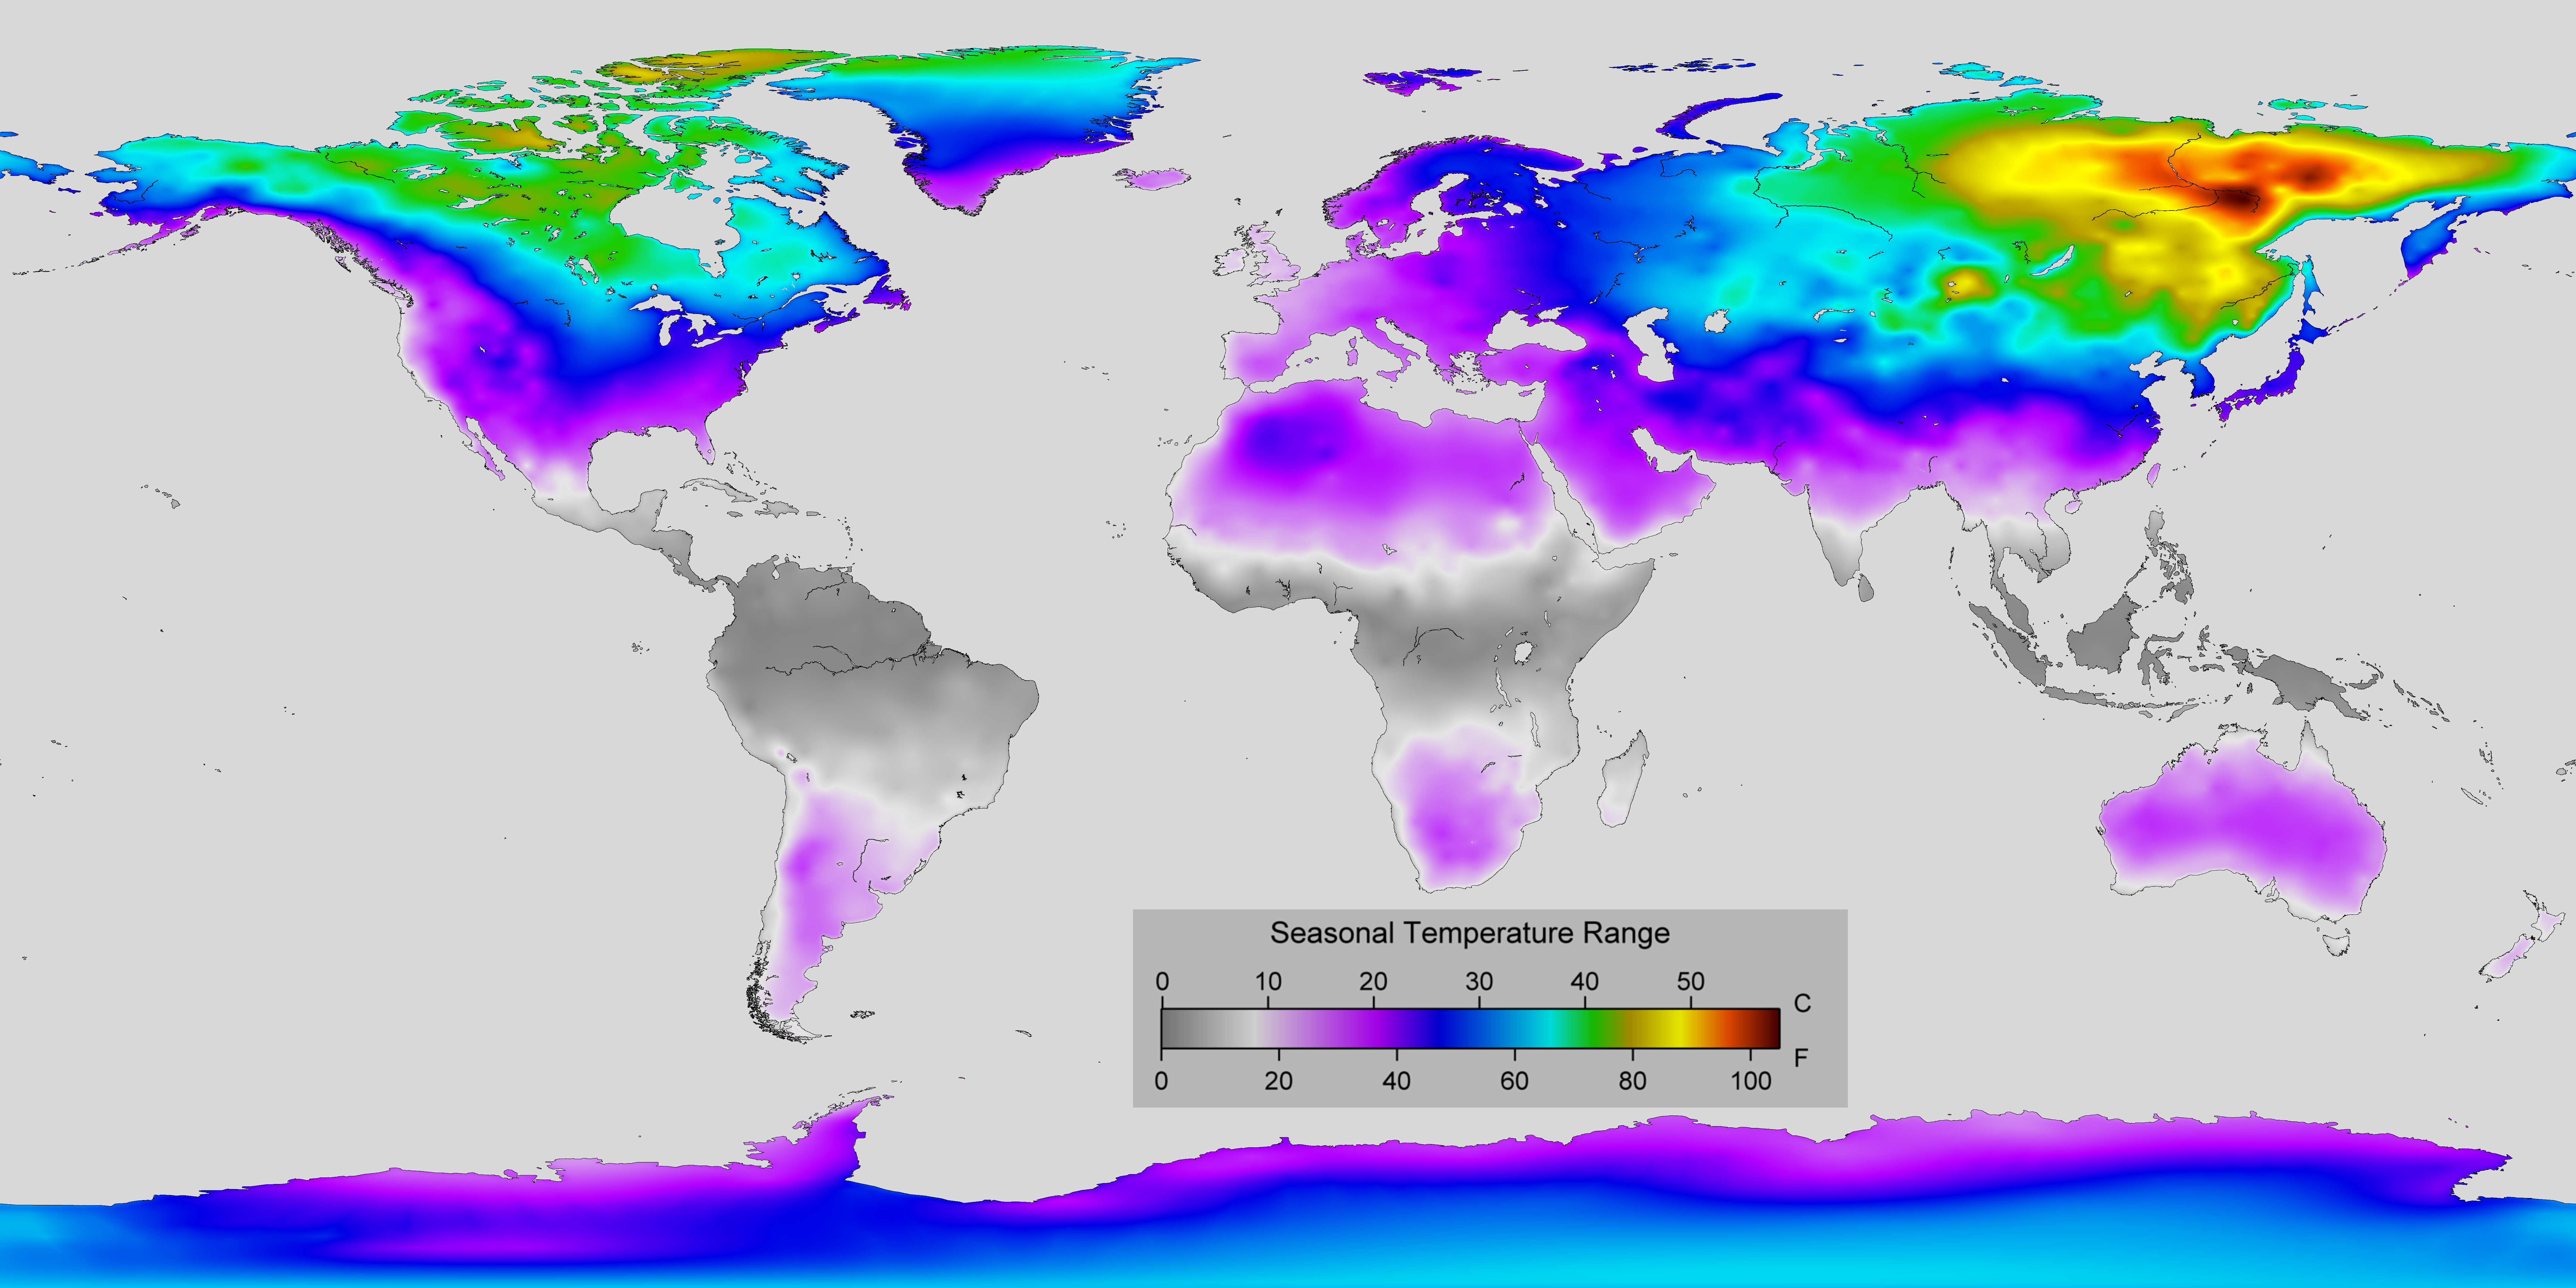
\includegraphics[width=\linewidth]{AVT.png}\\
      % {\tiny CC BY-SA 3.0, \url{https://commons.wikimedia.org/w/index.php?curid=3558400}\par}
   \end{center}
    
  \end{frame}

%%%%%%%%%%%%%%%%%%%%%%%%%%%%%%%%%%%%%%%%%%%%%%%%%%%%%%
\begin{frame}{The importance of temperature}

\begin{columns}[c]
    \column{0.3\textwidth}\centering
      \vspace*{\fill} 
      \includegraphics[width=\textwidth]{Darwin.jpg}\\
      {\tiny Public Domain, \url{https://commons.wikimedia.org/w/index.php?curid=11264065} \par} 
      \vspace*{\fill}
    \column{0.7\textwidth}
    \vspace*{\fill} 
    \begin{quote} 
      Climate plays an important part in determining the average numbers 
      of a species, and periodical seasons of extreme cold or drought seem 
      to be the most effective of all checks.\\
      \centering 
      \hfill -- {\small Darwin 1859, ``The origin of species''}
    \end{quote}
    \vspace*{\fill}
  \end{columns}

\end{frame}

%%%%%%%%%%%%%%%%%%%%%%%%%%%%%%%%%%%%%%%%%%%%%%%%%%%%%%
\begin{frame}{The importance of temperature}

  \begin{itemize}[<+->]\setlength{\itemindent}{0em}\itemsep10pt
    \item {\bf Recall what Metabolism is}: {\it Set of chemical reactions in a living organism}
    \item All chemical reactions are temperature-dependent: reaction rates increase with temperature
    \begin{itemize}
      \item An increase in temperature raises the average kinetic energy of reactant molecules
    \end{itemize}   
    \item This includes biochemical reactions, and enzyme activity
    \item The increase in biochemical reaction rate follows the {\it Boltzmann-Arrhenius equation}
    \item Therefore, metabolic rates go up (approximately) exponentially with temperature to a point and then decline: this is the ``Thermal Performance Curve''
  \end{itemize}
  
  \end{frame}

%%%%%%%%%%%%%%%%%%%%%%%%%%%%%%%%%%%%%%%%%%%%%%%%%%%%%
\begin{frame}{The importance of temperature}

  \begin{itemize}[<+->]\setlength{\itemindent}{-1em}\itemsep6pt
    \item These are a ``thermal performance curves'' of two bioluminescent bacteria ({\it A. fischeri} is symbiotic with squids) 
  \begin{columns}[c]
    \column{0.45\textwidth}\centering
      \includegraphics[width=\textwidth]{graphics/Photobacterium.pdf}
    \column{0.55\textwidth}
      \begin{itemize}\setlength{\itemindent}{-1em}
        \item The increase is due to increase in enzyme (e.g., luciferase) activity (following the Boltzmann-Arrhenius equation)
        \item The decline is because enzymes stop performing efficiently beyond some {\it optimal temperature} 
      \end{itemize} 
  \end{columns}

    \item Key biological rates---Respiration, photosynthesis, individual growth, etc.---all also depend upon temperature in a similar way
  \end{itemize}

\end{frame}

%%%%%%%%%%%%%%%%%%%%%%%%%%%%%%%%%%%%%%%%%%%%%%%%%%%%%%
\begin{frame}{The importance of temperature}

	\begin{itemize}
		\item The mechanistic basis of thermal performance curves (\url{https://youtu.be/6n8fCuDwn74}) 
	\end{itemize}

\begin{columns}[c]
  \column{.4\textwidth}
    \pause
      \includegraphics[width=\textwidth]{graphics/Photobacterium.pdf}
  \pause
  \column{.6\textwidth}
  \scriptsize
    $B = B_0 \boxed {e^{-\frac{E}{kT}}}f(T,T_{pk},E_D)$\\
    \vspace{10pt}
    \raggedright{$T$ = temperature (K)\\
     $k$ = Boltzmann constant (eV K$^{-1}$)}\\
     $E$ = Activation energy (eV)\\
     $T_{pk}$ = Temperature of peak performance\\
	 $E_D$ = Deactivation energy (eV)\\
	 
    {\tiny (J H van't Hoff 1884, S Arrhenius 1889)}
\end{columns}

\begin{itemize}\setlength{\itemindent}{0em}
  \pause
  \item But there is more to thermal responses
    \begin{itemize}\setlength{\itemindent}{-1em}
     \item Oxygen limitation
     \item Complexity of metabolic network
     \item Hormonal regulation
     \item Membrane fluidity
    \end{itemize}
    \pause
  \item \textit{Read Knapp \& Huang 2022 paper}\\

\end{itemize}
 
\end{frame}

%%%%%%%%%%%%%%%%%%%%%%%%%%%%%%%%%%%%%%%%%%%%%%%%%%%%%%
\begin{frame}{The ecological and evolutionary implications of temperature}

  \begin{columns}[c]
    \column{0.75\textwidth}\centering
    \begin{itemize}[<+->]\setlength{\itemindent}{0em}\itemsep4pt
      \item {\it Ectothermic organisms} (more accurately, {\it poikilotherms}) directly depend on the external temperature to get their ``engine running''   
      \item These are the {\it vast majority} of life on earth: Microbes, Plants, Insects, and many Vertebrates
    \end{itemize}
      \column{0.25\textwidth}
    \pause \includegraphics[width=\textwidth]{Lizard.JPG}
  \end{columns}
  \vspace{12pt}
  \pause
  \begin{columns}[c]
    \column{0.75\textwidth}\centering
    \begin{itemize}[<+->]\setlength{\itemindent}{0em}\itemsep4pt
      \item {\it Endothermic organisms} keep their ``engine running'' by generating their own heat
      \item These are are {\it minuscule minority} of life on earth: Basically, Mammals and Birds
    \end{itemize}
      \column{0.25\textwidth}
    \pause \includegraphics[width=\textwidth]{Hummer.jpg}
  \end{columns}
  
  \end{frame}

%%%%%%%%%%%%%%%%%%%%%%%%%%%%%%%%%%%%%%%%%%%%%%%%%%%%%%
\begin{frame}{The ecological implications of temperature}

  \begin{center}
    \includegraphics[width=0.8\textwidth]{Bar-on_et_al.pdf}\\
    {\tiny Bar-On et al, ``The Biomass Distribution on Earth'' PNAS 2018}
  \end{center}\par

  \begin{itemize}[<+->]\setlength{\itemindent}{0em}\itemsep4pt
      \item Metabolic rates of the {\it vast majority} of life depend directly on environmental temperature
      \item The rest, endotherms, also depend indirectly on temperature (e.g., they eat ectotherms -- rabbit eating grass)
      \item Population growth rates also increase with temperature (to a point - remember the Thermal Performance Curve)
  \end{itemize}

  \end{frame}

%%%%%%%%%%%%%%%%%%%%%%%%%%%%%%%%%%%%%%%%%%%%%%%%%%%%%%
\section{\scshape Summary}
% \subsection{}
   
%%%%%%%%%%%%%%%%%%%%%%%%%%%%%%%%%%%%%%%%%%%%%%%%%%%%%%

\begin{frame}{Summary}

  \begin{itemize}[<+->] \setlength{\itemindent}{0em} \itemsep10pt
  
      \item Individual metabolism drives individual and population growth rate
      
      \item Metabolic rate increases as a power-law with size 
  
      \begin{itemize}
        \item  Thus, size determines population growth rate and population size
      \end{itemize}

      \item  Metabolic rate increases (approximately) exponentially with temperature (to a point)
      
      \begin{itemize}
        \item Thus, temperature also determines population growth rate and population size
      \end{itemize}
  
      \item {\it Between metabolic rate and production ($r_{max}$), lies 
       consumption --- what must consumption rate scale like?} (Next lecture)
  
  \end{itemize}  
  
  \end{frame}

  
%%%%%%%%%%%%%%%%%%%%%%%%%%%%%%%%%%%%%%%%%%%%%%%%%%%%%%
  \begin{frame}{Readings}
    \begin{enumerate}\setlength{\itemindent}{-2em}\itemsep4pt
  \small
    % \item Kleiber, M. Body size and metabolic rate. Physiological Reviews 27, 
    % 511--541 (1947).
    
    \item West, G. B. \& Brown, J. H. The origin of allometric scaling laws in
    biology from genomes to ecosystems: towards a quantitative unifying theory of biological structure and organization. Journal of Experimental Biology 208, 1575–92 (2005).
    
    % \item Ballesteros, F. J. et al. On the thermodynamic origin of metabolic
    % scaling. Scientific Reports 8, 1448 (2018).
      
    \item Brown, J. H., et al. Toward a metabolic theory of ecology. Ecology 85,
    1771--1789 (2004). 
    
    \item Knapp B. D., \& Huang K. C. The Effects of Temperature on Cellular
    Physiology. Annu Rev Biophys 51, 499--526 (2022).

    \item Dell, A. I., Pawar, S. \& Savage, V. M. Systematic variation in the
    temperature dependence of physiological and ecological traits. PNAS 108,
    10591--10596 (2011).
  
    \item Arroyo, José Ignacio, Beatriz Díez, Christopher P. Kempes, Geoffrey B. West, \& Pablo A. Marquet. "A general theory for temperature dependence in biology." Proceedings of the National Academy of Sciences 119, no. 30 (2022): e2119872119.
  
    \end{enumerate}
  
\end{frame}

%%%%%%%%%%%%%%%%%%%%%%%%%%%%%%%%%%%%%%%%%%%%%%%%%%%%%%
\begin{frame}{Practicals}
  
  \begin{enumerate}\setlength{\itemindent}{-2em}\itemsep2pt

    \item Review ``Making mathematical statements'' section of the MQB's \emph{Maths for Biologists Appendix}: \url{https://mulquabio.github.io/MQB/notebooks/Appendix-MathsForBiologists/MathsForBiologists.html}
    
    \item Solve problems 1-3 of the Exercise set 1 of ``Maths for Biologists'' Appendix: \url{https://mulquabio.github.io/MQB/notebooks/Appendix-MathsForBiologists/MathsForBiologists.html}
    
    \item Read and work through to the end of ``Some preliminaries'' section of \emph{Mathematical models in Jupyter Appendix}: \url{https://mulquabio.github.io/MQB/notebooks/Appendix-Maths.html}
    % 
  \end{enumerate}
  
\end{frame}

%%%%%%%%%%%%%%%%%%%%%%%%%%%%%%%%%%%%%%%%%%%%%%%%%%%%%%
\begin{frame}{Discussion Questions}

  \begin{enumerate}\setlength{\itemindent}{-2em}\itemsep3pt
  
    \item Given the way resting metabolic rate scales with body size, what must consumption rate scale like?
    
    \item Why did we focus on {\it resting} (or ``basal'') metabolic rate?

    \item How much energy would a {\it resting} rabbit ($\sim 1$ kg), a human ($\sim 70$ kg, and an Asian elephant ($\sim 4000$ kg) need for metabolic balance\footnotemark,
    \begin{itemize}
      \item at the individual level?
      \item per unit mass?
    \end{itemize}
    \footnotetext{Calculate it using Kleiber's law (allometric/scaling equation), as we did for a mouse}

    \item How does the value you calculated in the previous question compare with the recommended calorie intake for humans? Is it lower or higher? Why?  

    \item What are the optimal temperatures for the enzyme underlying bioluminescence in the two bacteria in the given example? Why might they have different thermal optima? 

  \end{enumerate}
  
\end{frame}

\end{document}
